\documentclass{report}

% Packages
\usepackage{lipsum} % For generating dummy text
\usepackage{graphicx} % For including images
\usepackage{cite} % For citations
\usepackage{hyperref} % For hyperlinks

% Title page information
\title{InfiniTerra: An Infinite Terrain Generation System}
\author{Mirto Randellini}
\date{\today}

\begin{document}

% Title page
\maketitle

% Table of contents
\tableofcontents

% Abstract
\begin{abstract}
This is the abstract of my report.
\end{abstract}

% Introduction
\chapter{Introduction}
\label{ch:introduction}
% Why make an infinite terrain?
Infinite terrains are a common feature in video games and other real-time applications, like flight simulators and virtual reality experiences.
They allow for the creation of vast, open worlds that players can explore without encountering any boundaries.
This can enhance the sense of immersion and freedom in a game, as players can travel in any direction without being constrained by the size of the game world.
In this report, we will discuss the design and implementation of an infinite terrain generation system called InfiniTerra.
We will cover the theory behind terrain generation, the algorithms used to generate the terrain, and the rendering techniques used to display the terrain to the player.
We will also discuss the challenges of creating an infinite terrain system and how they were overcome in the development of InfiniTerra.
% Relevant existing work in games
Before diving into the details of the system, it is interesting to mention some of the existing work in the field of terrain generation.
The earliest use of procedural generation in games can be traced back to the 1980s, with games like \textit{Hack} and \textit{Rogue}.
These games used procedural generation to create dungeons and levels that were different each time the player played the game and they spawned a whole genre of games known as roguelikes.

\begin{figure}[h!]
  \centering
  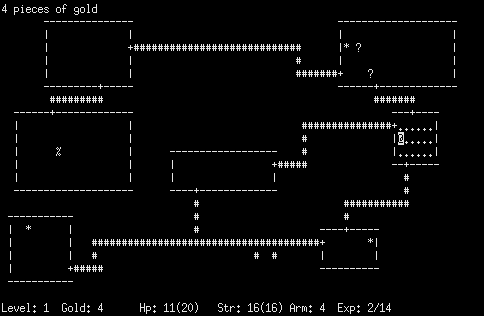
\includegraphics[width=0.75\textwidth]{img/rogue.png}
  \caption{A procedurally generated dungeon map in the videogame Rogue.}
  \label{fig:nethack}
\end{figure}

Moving forward to 1996, the game \textit{Elder Scrolls II: Daggerfall} featured a procedurally generated world with a size of 161,600 square kilometers (approximately the size of England), which was the largest game world ever created at the time, and it is still one of the largest game worlds ever created.
To be precise the wilderness between locations is based on a rudimentary heightmap, one pixel of which covers 800 in-game metres.
Smaller details are randomly generated, while actual locations are pre-generated, and are consequently always the same.

\begin{figure}[h!]
  \centering
  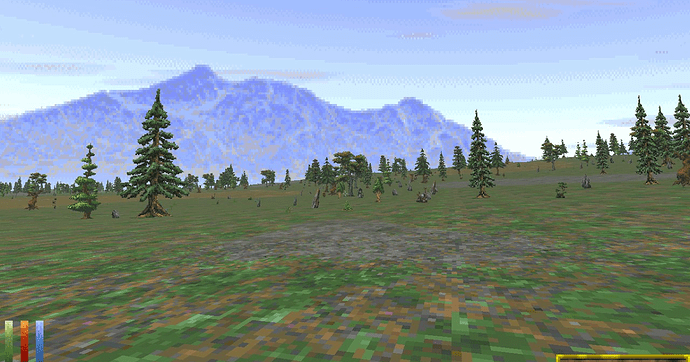
\includegraphics[width=0.75\textwidth]{img/daggerfall.png}
  \caption{The procedurally generated world map of the game Elder Scrolls II: Daggerfall.}
  \label{fig:daggerfall}
\end{figure}

Today one of the most famous examples of procedural generation in games is \textit{Minecraft}, a game that features a procedurally generated world made up of blocks that players can mine and place to create their own structures.
The world in Minecraft is generated using Perlin noise, a type of gradient noise that is commonly used in procedural generation to create natural-looking terrains.
The generation algorithm has then been improved over the years to include more complex features like caves, villages, and biomes.

\begin{figure}[h!]
  \centering
  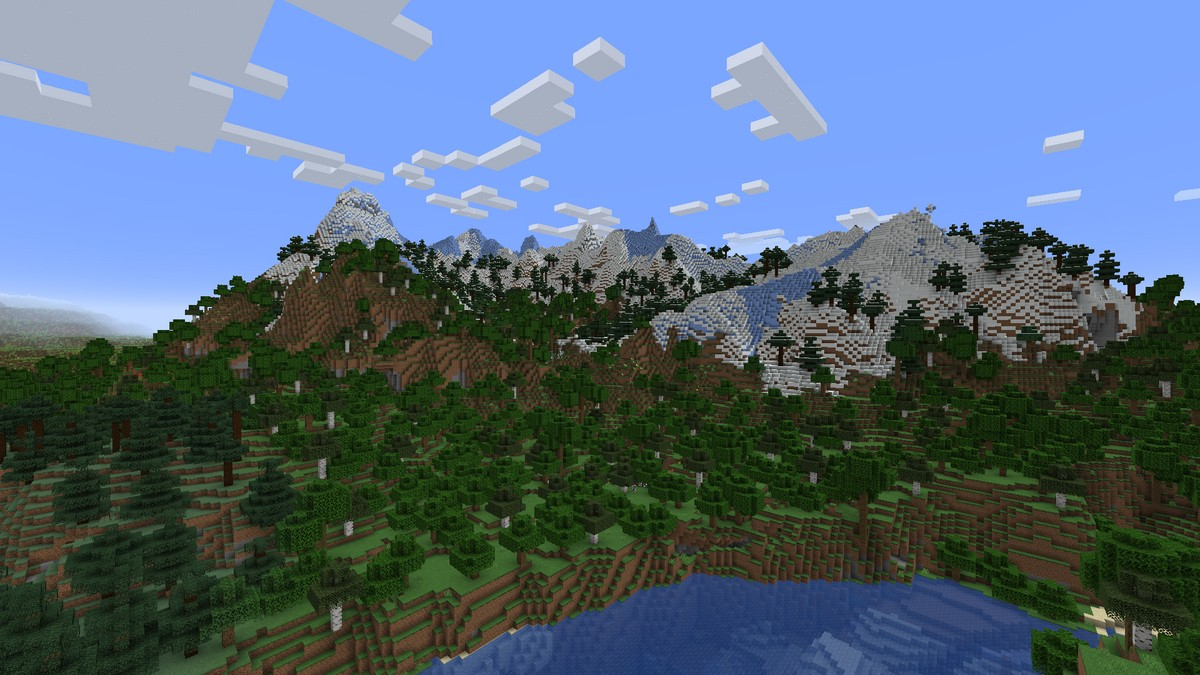
\includegraphics[width=0.75\textwidth]{img/minecraft.jpg}
  \caption{A procedurally generated world in the videogame Minecraft.}
  \label{fig:minecraft}
\end{figure}

%End introduction


\chapter{Generating the terrain}
\label{ch:generating-the-terrain}
% Heightmap generation
Commonly used techniques for terrain generation include heightmap generation, fractal terrain generation, and procedural generation using noise functions.
These techniques use mathematical functions to generate terrain data that can be used to displace the vertices of a grid to create a 3D terrain.
In InfiniTerra, we use a heightmap generation technique based on ridged Perlin noise to create the terrain.
% Perlin noise
\section*{Perlin Noise}
Perlin noise is a type of gradient noise developed by Ken Perlin in 1983. It is commonly used in computer graphics to create natural-looking textures and terrains.
Interestingly it's first use was in the movie Tron (1982) to create the light cycle effects.
% CPU implementation
\subsection*{CPU Implementation}
In the first version of the system, the heightmap generation was implemented on the CPU by using the FastNoiseLite library.
This allowed access to a wide variety of noise functions, such as Perlin, Simplex, and Cellular noise, but was not performant enough for generating large terrains.
The generation of a 1024x1024 heightmap took around 5s on a modern CPU, which was too slow for real-time applications.
% GPU implementation (compute shaders)
\subsection*{GPU Implementation}
To improve performance, the heightmap generation was moved to the GPU by using compute shaders.

\section*{Compute shaders}
% Introduce the pipeline and shader stages
In modern graphics programming, the rendering pipeline is divided into several stages, each of which is implemented using a different type of shader.

\begin{figure}[h!]
  \centering
  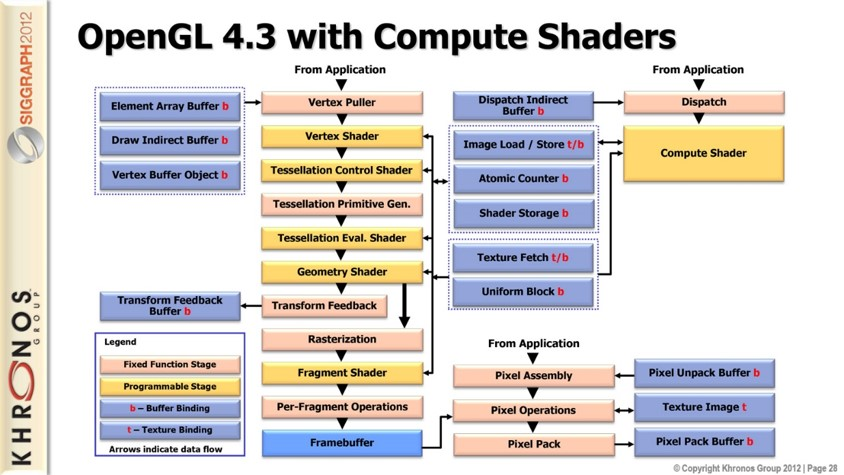
\includegraphics[width=0.75\textwidth]{img/compute_shaders.jpg}
  \caption{The graphics rendering pipeline.}
  \label{fig:pipeline}
\end{figure}

A Compute Shader is a shader stage that is used entirely for computing arbitrary information. While it can do rendering, it is generally used for tasks not directly related to drawing triangles and pixels.
It is used to perform general-purpose computing tasks on the GPU, such as physics simulations, image processing, and data processing.
The compute shader is executed in parallel by multiple threads, which allows it to perform computations much faster than the CPU.
Compute shaders are not part of the regular rendering pipeline. So when executing a Drawing Command, the compute shader linked into the current program or pipeline is not involved. Instead, you must explicitly dispatch a compute shader to run on the GPU.
Compute shaders operate in an abstracted space called a dispatch grid, which is a 3D grid of thread groups. We call these groups \textit{work groups}.
When the system actually computes the work groups, it can do so in any order. So if it is given a work group set of (3, 1, 2), it could execute group (0, 0, 0) first, then skip to group (1, 0, 1), then jump to (2, 0, 0), etc. So your compute shader should not rely on the order in which individual groups are processed.
A single work group is not the same thing as a single compute shader invocation; there's a reason why it is called a \textit{group}. Within a single work group, there may be many compute shader invocations. How many is defined by the compute shader itself, not by the call that executes it. This is known as the local size of the work group. 
Each thread group contains multiple threads, which can communicate with each other using shared memory. This allows the compute shader to perform complex computations that require synchronization between threads.
A compute shader doesn't have access to the same inputs and outputs as other shader stages, but it can read and write to buffers and textures, which allows it to perform a wide variety of computations.

\chapter{Rendering the terrain}
\label{ch:rendering-the-terrain}
% Base geometry (triangles)
% Phong Lighting
\section{Phong Lighting}
% Phong lighting theory
Phong lighting is a shading model developed by Bui Tuong Phong in 1975. It is a local illumination model that approximates the way light interacts with a surface by using three components: ambient, diffuse, and specular.
The ambient component represents the light that is scattered in all directions and is reflected equally by all surfaces.
The diffuse component represents the light that is scattered in all directions but is reflected more in the direction of the light source.
The specular component represents the light that is reflected in a specific direction, which is determined by the angle between the light source and the viewer.
% Phong lighting implementation

% Chunking and culling
\section*{Chunking and Culling}
% LOD (tessellation)
\section*{Level of Detail (LOD)}
Level of Detail (LOD) is a technique used in computer graphics to optimize the rendering of complex 3D models by reducing the level of detail based on the distance from the camera.
This allows the rendering engine to display high-quality models when they are close to the camera and switch to lower-quality models when they are far away.
In InfiniTerra, we use an LOD system based on tessellation to dynamically adjust the level of detail of the terrain based on the distance from the camera.
This is done by subdividing the terrain into smaller patches and increasing the level of tessellation as the camera gets closer to the terrain.
This affords us multi-resolution control over every chunk of terrain, allowing the same mesh to be rendered with different levels of detail depending on the distance from the camera.
\section*{Tessellation}
Tessellation is the Vertex Processing stage in the OpenGL rendering pipeline where patches of vertex data are subdivided into smaller Primitives. This process is governed by two shader stages and a fixed-function stage. 
\lipsum[3-4]

% Conclusion
\chapter{Conclusion}
\label{ch:conclusion}
\lipsum[7-8]

% References
\bibliographystyle{plain}
\bibliography{references}

\end{document}